\documentclass[14pt]{extbook}
\usepackage{multicol, enumerate, enumitem, hyperref, color, soul, setspace, parskip, fancyhdr} %General Packages
\usepackage{amssymb, amsthm, amsmath, latexsym, units, mathtools} %Math Packages
\everymath{\displaystyle} %All math in Display Style
% Packages with additional options
\usepackage[headsep=0.5cm,headheight=12pt, left=1 in,right= 1 in,top= 1 in,bottom= 1 in]{geometry}
\usepackage[usenames,dvipsnames]{xcolor}
\usepackage{dashrule}  % Package to use the command below to create lines between items
\newcommand{\litem}[1]{\item#1\hspace*{-1cm}\rule{\textwidth}{0.4pt}}
\pagestyle{fancy}
\lhead{Progress Quiz 4}
\chead{}
\rhead{Version ALL}
\lfoot{5346-5907}
\cfoot{}
\rfoot{Summer C 2021}
\begin{document}

\begin{enumerate}
\litem{
Choose the equation of the function graphed below.
\begin{center}
    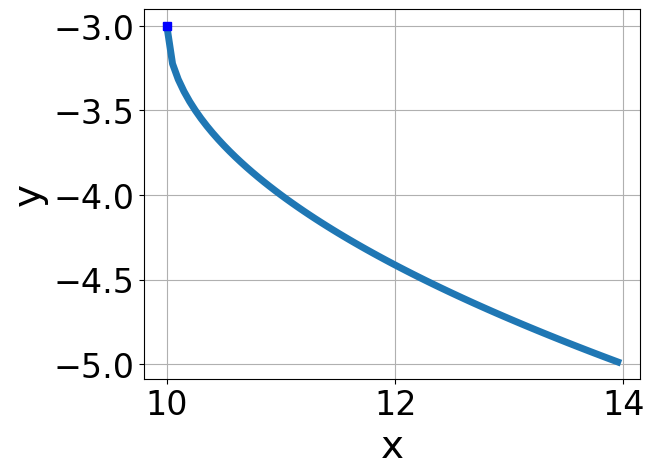
\includegraphics[width=0.5\textwidth]{../Figures/radicalGraphToEquationA.png}
\end{center}
\begin{enumerate}[label=\Alph*.]
\item \( f(x) = - \sqrt{x + 10} - 3 \)
\item \( f(x) = \sqrt{x + 10} - 3 \)
\item \( f(x) = - \sqrt{x - 10} - 3 \)
\item \( f(x) = \sqrt{x - 10} - 3 \)
\item \( \text{None of the above} \)

\end{enumerate} }
\litem{
Choose the graph of the equation below.\[ f(x) = \sqrt[3]{x - 6} + 4 \]\begin{enumerate}[label=\Alph*.]
\begin{multicols}{2}\item 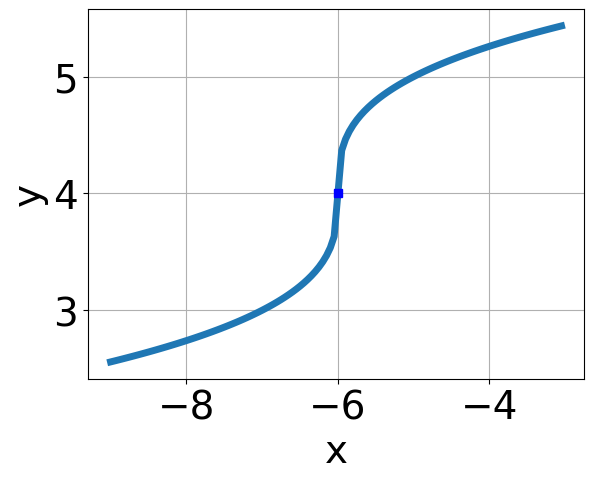
\includegraphics[width = 0.3\textwidth]{../Figures/radicalEquationToGraphCopyAA.png}\item 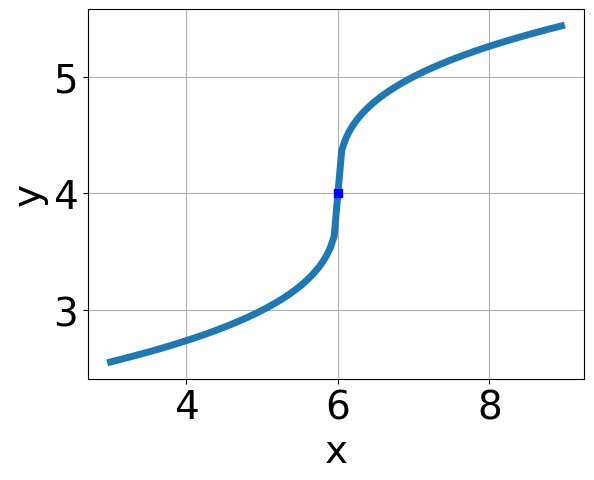
\includegraphics[width = 0.3\textwidth]{../Figures/radicalEquationToGraphCopyBA.png}\item 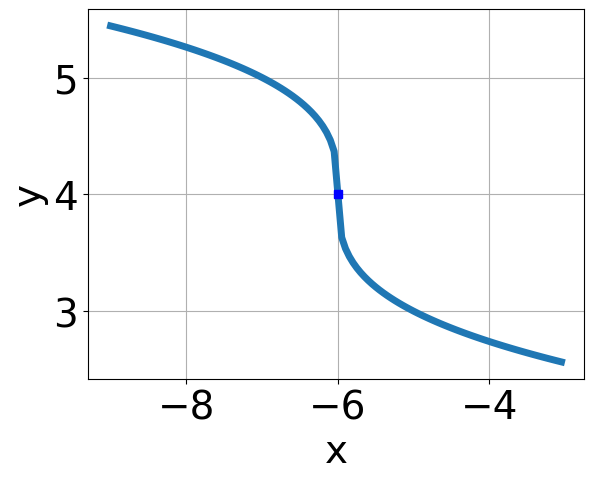
\includegraphics[width = 0.3\textwidth]{../Figures/radicalEquationToGraphCopyCA.png}\item 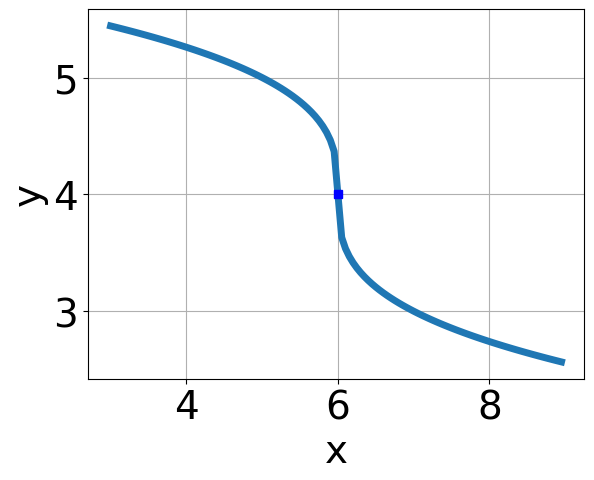
\includegraphics[width = 0.3\textwidth]{../Figures/radicalEquationToGraphCopyDA.png}\end{multicols}\item None of the above.
\end{enumerate} }
\litem{
Choose the graph of the equation below.\[ f(x) = \sqrt{x + 10} + 3 \]\begin{enumerate}[label=\Alph*.]
\begin{multicols}{2}\item 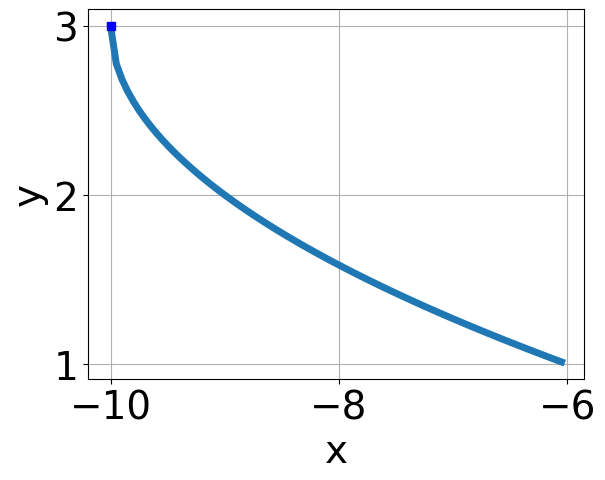
\includegraphics[width = 0.3\textwidth]{../Figures/radicalEquationToGraphAA.png}\item 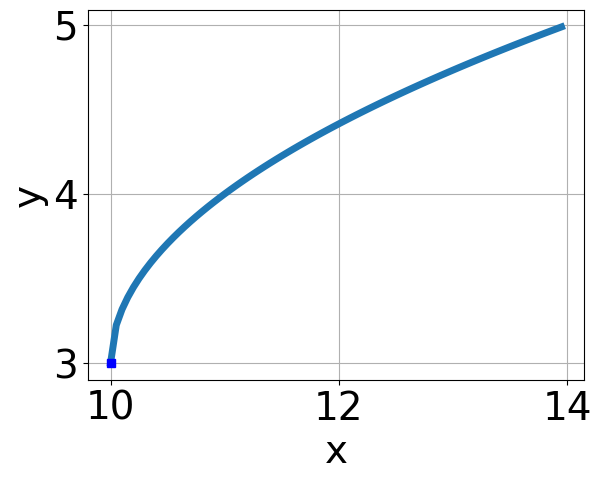
\includegraphics[width = 0.3\textwidth]{../Figures/radicalEquationToGraphBA.png}\item 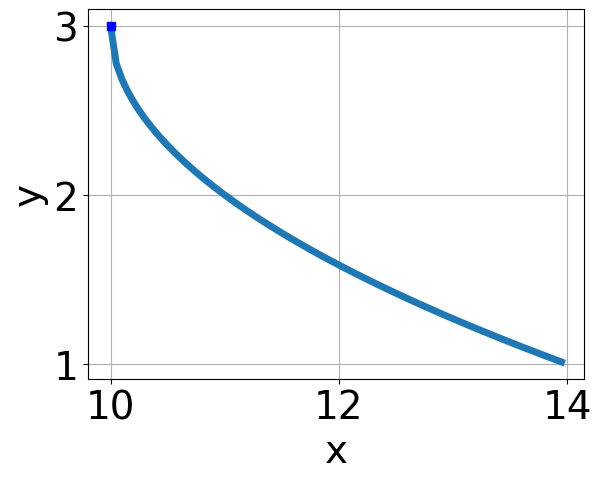
\includegraphics[width = 0.3\textwidth]{../Figures/radicalEquationToGraphCA.png}\item 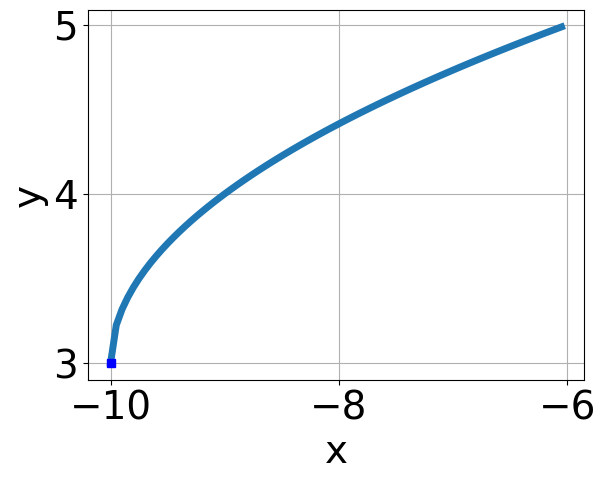
\includegraphics[width = 0.3\textwidth]{../Figures/radicalEquationToGraphDA.png}\end{multicols}\item None of the above.
\end{enumerate} }
\litem{
Solve the radical equation below. Then, choose the interval(s) that the solution(s) belongs to.\[ \sqrt{48 x^2 - 30} - \sqrt{-4 x} = 0 \]\begin{enumerate}[label=\Alph*.]
\item \( x \in [-2.83,0.17] \)
\item \( x \in [-0.25,3.75] \)
\item \( \text{All solutions lead to invalid or complex values in the equation.} \)
\item \( x_1 \in [-0.25, 3.75] \text{ and } x_2 \in [0.79,0.87] \)
\item \( x_1 \in [-2.83, 0.17] \text{ and } x_2 \in [0.67,0.76] \)

\end{enumerate} }
\litem{
Solve the radical equation below. Then, choose the interval(s) that the solution(s) belongs to.\[ \sqrt{9 x + 5} - \sqrt{5 x + 5} = 0 \]\begin{enumerate}[label=\Alph*.]
\item \( x \in [-2.98,-1.79] \)
\item \( x_1 \in [-1.09, -0.92] \text{ and } x_2 \in [-0.87,-0.55] \)
\item \( x_1 \in [-0.63, -0.24] \text{ and } x_2 \in [-0.55,0.11] \)
\item \( x \in [-0.45,0.4] \)
\item \( \text{All solutions lead to invalid or complex values in the equation.} \)

\end{enumerate} }
\litem{
Choose the equation of the function graphed below.
\begin{center}
    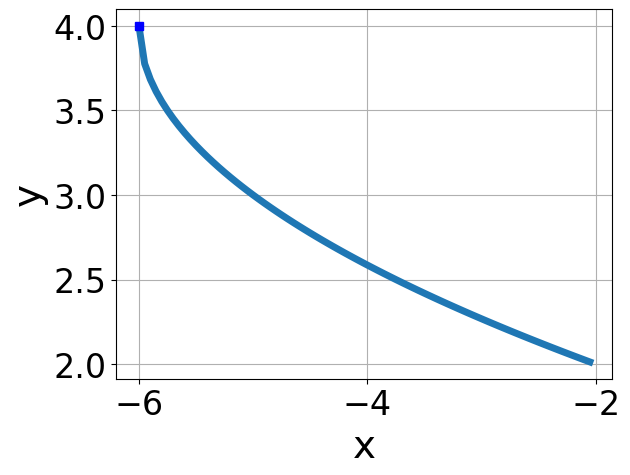
\includegraphics[width=0.5\textwidth]{../Figures/radicalGraphToEquationCopyA.png}
\end{center}
\begin{enumerate}[label=\Alph*.]
\item \( f(x) = - \sqrt{x + 6} + 4 \)
\item \( f(x) = \sqrt{x - 6} + 4 \)
\item \( f(x) = \sqrt{x + 6} + 4 \)
\item \( f(x) = - \sqrt{x - 6} + 4 \)
\item \( \text{None of the above} \)

\end{enumerate} }
\litem{
Solve the radical equation below. Then, choose the interval(s) that the solution(s) belongs to.\[ \sqrt{-24 x^2 + 21} - \sqrt{10 x} = 0 \]\begin{enumerate}[label=\Alph*.]
\item \( \text{All solutions lead to invalid or complex values in the equation.} \)
\item \( x \in [-1.29,-0.35] \)
\item \( x_1 \in [-1.29, -0.35] \text{ and } x_2 \in [0.64,0.94] \)
\item \( x_1 \in [0.44, 1.41] \text{ and } x_2 \in [0.96,1.3] \)
\item \( x \in [0.44,1.41] \)

\end{enumerate} }
\litem{
Solve the radical equation below. Then, choose the interval(s) that the solution(s) belongs to.\[ \sqrt{-3 x + 2} - \sqrt{-6 x + 7} = 0 \]\begin{enumerate}[label=\Alph*.]
\item \( \text{All solutions lead to invalid or complex values in the equation.} \)
\item \( x \in [1.08,1.84] \)
\item \( x_1 \in [-0.34, 0.84] \text{ and } x_2 \in [1.4,2] \)
\item \( x \in [-3.15,-1.87] \)
\item \( x_1 \in [-0.34, 0.84] \text{ and } x_2 \in [0.2,1.6] \)

\end{enumerate} }
\litem{
What is the domain of the function below?\[ f(x) = \sqrt[3]{-4 x + 9} \]\begin{enumerate}[label=\Alph*.]
\item \( \text{The domain is } (-\infty, a], \text{   where } a \in [-2.6, 0.5] \)
\item \( \text{The domain is } (-\infty, a], \text{   where } a \in [1.3, 2.8] \)
\item \( \text{The domain is } [a, \infty), \text{   where } a \in [1.2, 2.7] \)
\item \( (-\infty, \infty) \)
\item \( \text{The domain is } [a, \infty), \text{   where } a \in [-1.4, 1.6] \)

\end{enumerate} }
\litem{
What is the domain of the function below?\[ f(x) = \sqrt[4]{7 x + 3} \]\begin{enumerate}[label=\Alph*.]
\item \( [a, \infty), \text{ where } a \in [-2.2, 1.3] \)
\item \( (-\infty, \infty) \)
\item \( (-\infty, a], \text{where } a \in [-3.5, -0.5] \)
\item \( [a, \infty), \text{where } a \in [-5.8, -2.2] \)
\item \( (-\infty, a], \text{where } a \in [-1.6, 0.1] \)

\end{enumerate} }
\litem{
Choose the equation of the function graphed below.
\begin{center}
    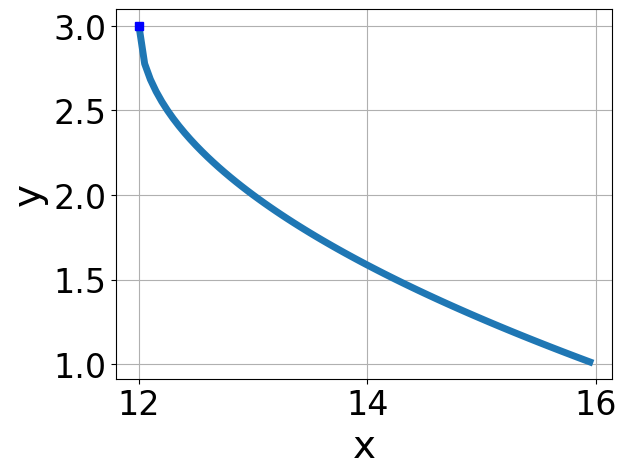
\includegraphics[width=0.5\textwidth]{../Figures/radicalGraphToEquationB.png}
\end{center}
\begin{enumerate}[label=\Alph*.]
\item \( f(x) = \sqrt[3]{x + 12} + 3 \)
\item \( f(x) = - \sqrt[3]{x - 12} + 3 \)
\item \( f(x) = - \sqrt[3]{x + 12} + 3 \)
\item \( f(x) = \sqrt[3]{x - 12} + 3 \)
\item \( \text{None of the above} \)

\end{enumerate} }
\litem{
Choose the graph of the equation below.\[ f(x) = - \sqrt{x - 8} - 7 \]\begin{enumerate}[label=\Alph*.]
\begin{multicols}{2}\item 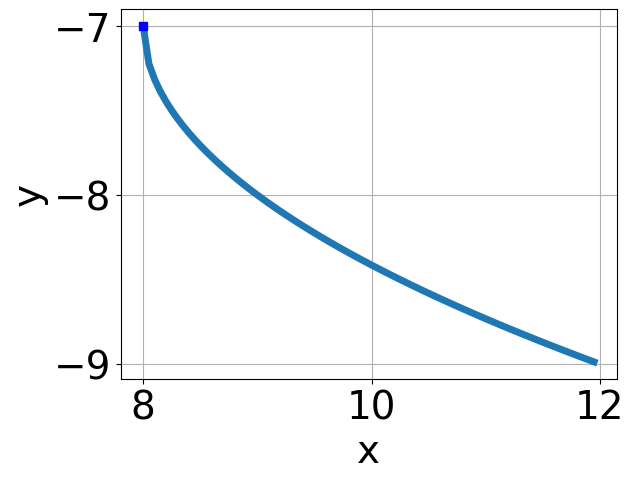
\includegraphics[width = 0.3\textwidth]{../Figures/radicalEquationToGraphCopyAB.png}\item 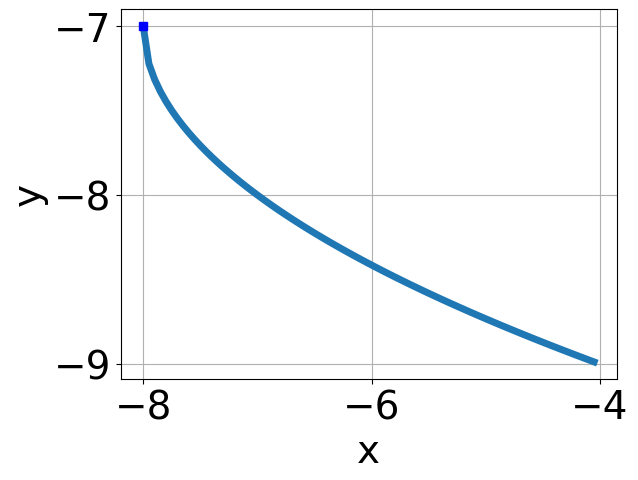
\includegraphics[width = 0.3\textwidth]{../Figures/radicalEquationToGraphCopyBB.png}\item 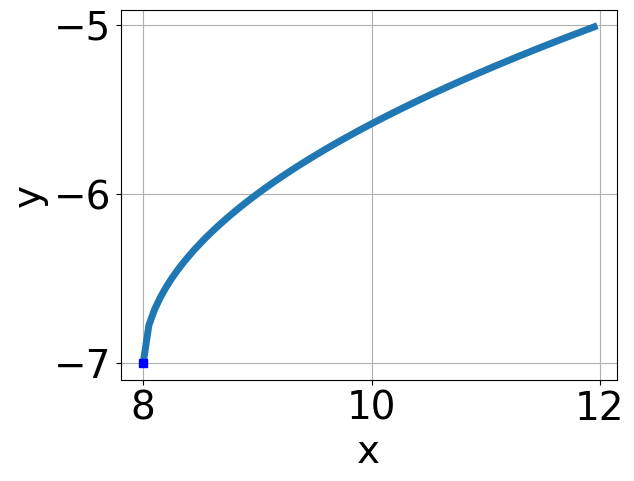
\includegraphics[width = 0.3\textwidth]{../Figures/radicalEquationToGraphCopyCB.png}\item 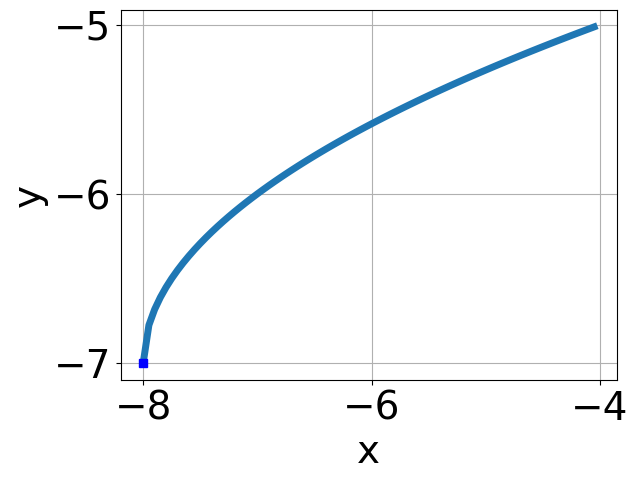
\includegraphics[width = 0.3\textwidth]{../Figures/radicalEquationToGraphCopyDB.png}\end{multicols}\item None of the above.
\end{enumerate} }
\litem{
Choose the graph of the equation below.\[ f(x) = \sqrt{x + 14} - 5 \]\begin{enumerate}[label=\Alph*.]
\begin{multicols}{2}\item 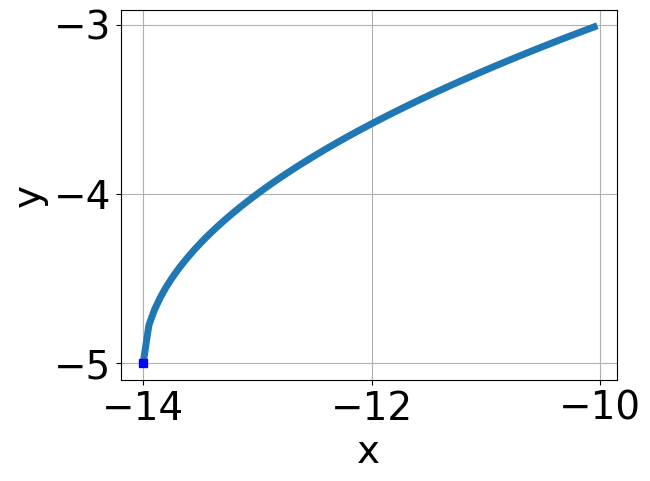
\includegraphics[width = 0.3\textwidth]{../Figures/radicalEquationToGraphAB.png}\item 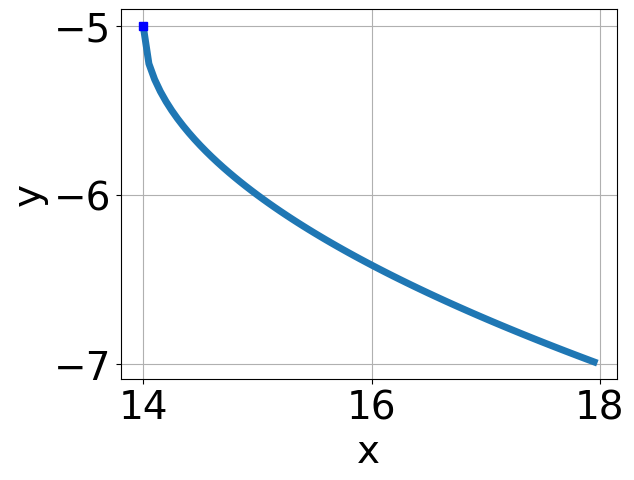
\includegraphics[width = 0.3\textwidth]{../Figures/radicalEquationToGraphBB.png}\item 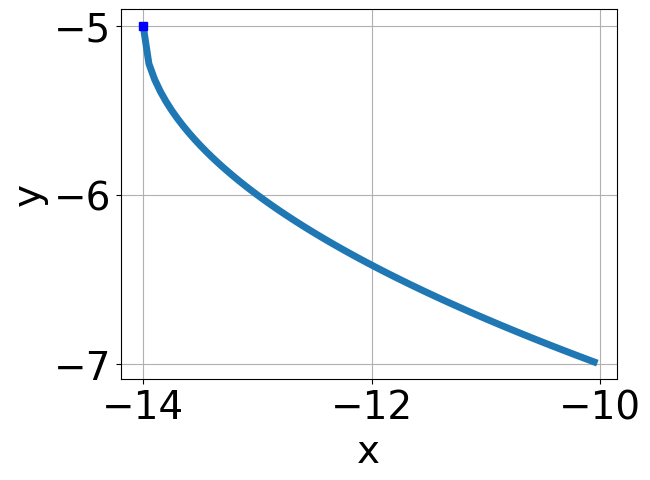
\includegraphics[width = 0.3\textwidth]{../Figures/radicalEquationToGraphCB.png}\item 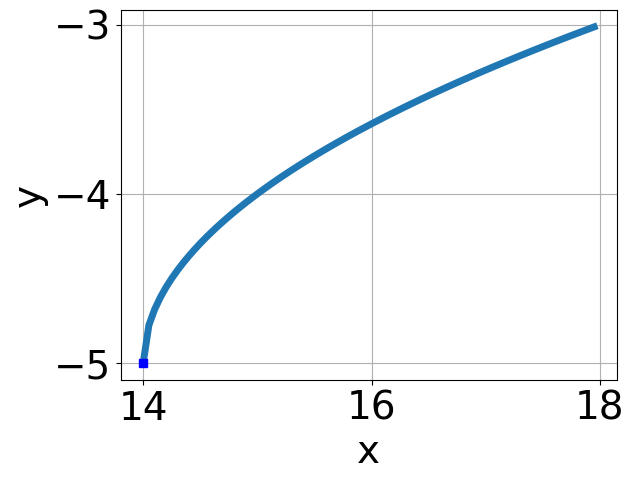
\includegraphics[width = 0.3\textwidth]{../Figures/radicalEquationToGraphDB.png}\end{multicols}\item None of the above.
\end{enumerate} }
\litem{
Solve the radical equation below. Then, choose the interval(s) that the solution(s) belongs to.\[ \sqrt{-9 x^2 - 15} - \sqrt{24 x} = 0 \]\begin{enumerate}[label=\Alph*.]
\item \( \text{All solutions lead to invalid or complex values in the equation.} \)
\item \( x_1 \in [1.62, 1.72] \text{ and } x_2 \in [-0.1,3.5] \)
\item \( x \in [-1.13,-0.71] \)
\item \( x \in [-1.83,-1.09] \)
\item \( x_1 \in [-1.83, -1.09] \text{ and } x_2 \in [-3.3,0.8] \)

\end{enumerate} }
\litem{
Solve the radical equation below. Then, choose the interval(s) that the solution(s) belongs to.\[ \sqrt{3 x - 6} - \sqrt{7 x + 5} = 0 \]\begin{enumerate}[label=\Alph*.]
\item \( x_1 \in [-0.81, -0.31] \text{ and } x_2 \in [1,4] \)
\item \( x \in [-3.45,-2.19] \)
\item \( x \in [-0.25,-0.06] \)
\item \( x_1 \in [-3.45, -2.19] \text{ and } x_2 \in [1,4] \)
\item \( \text{All solutions lead to invalid or complex values in the equation.} \)

\end{enumerate} }
\litem{
Choose the equation of the function graphed below.
\begin{center}
    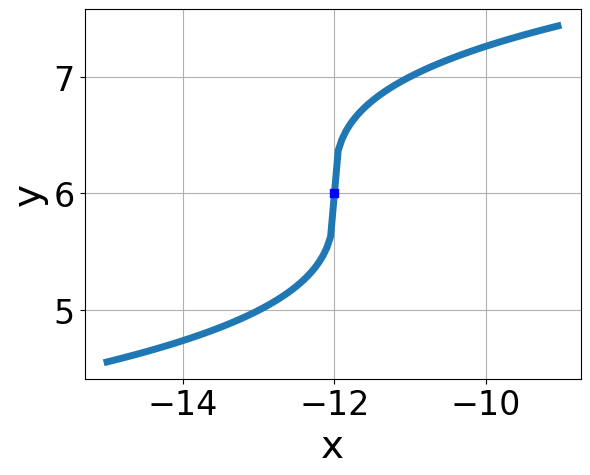
\includegraphics[width=0.5\textwidth]{../Figures/radicalGraphToEquationCopyB.png}
\end{center}
\begin{enumerate}[label=\Alph*.]
\item \( f(x) = - \sqrt[3]{x - 12} + 6 \)
\item \( f(x) = - \sqrt[3]{x + 12} + 6 \)
\item \( f(x) = \sqrt[3]{x - 12} + 6 \)
\item \( f(x) = \sqrt[3]{x + 12} + 6 \)
\item \( \text{None of the above} \)

\end{enumerate} }
\litem{
Solve the radical equation below. Then, choose the interval(s) that the solution(s) belongs to.\[ \sqrt{-16 x^2 - 45} - \sqrt{-58 x} = 0 \]\begin{enumerate}[label=\Alph*.]
\item \( x \in [2.1,3.1] \)
\item \( \text{All solutions lead to invalid or complex values in the equation.} \)
\item \( x_1 \in [0.6, 1.2] \text{ and } x_2 \in [2.5,3.5] \)
\item \( x \in [0.6,1.2] \)
\item \( x_1 \in [-1.9, -0.7] \text{ and } x_2 \in [-3.5,1.5] \)

\end{enumerate} }
\litem{
Solve the radical equation below. Then, choose the interval(s) that the solution(s) belongs to.\[ \sqrt{3 x + 4} - \sqrt{-9 x + 7} = 0 \]\begin{enumerate}[label=\Alph*.]
\item \( x_1 \in [-2.5, -1.27] \text{ and } x_2 \in [-0.21,0.62] \)
\item \( x \in [-0.67,1.18] \)
\item \( x_1 \in [-2.5, -1.27] \text{ and } x_2 \in [0.5,0.91] \)
\item \( \text{All solutions lead to invalid or complex values in the equation.} \)
\item \( x \in [-1.12,-0.11] \)

\end{enumerate} }
\litem{
What is the domain of the function below?\[ f(x) = \sqrt[4]{8 x - 7} \]\begin{enumerate}[label=\Alph*.]
\item \( (-\infty, \infty) \)
\item \( (-\infty, a], \text{where } a \in [1.05, 1.54] \)
\item \( (-\infty, a], \text{where } a \in [0.46, 1.03] \)
\item \( [a, \infty), \text{where } a \in [1.13, 1.28] \)
\item \( [a, \infty), \text{ where } a \in [0.71, 0.89] \)

\end{enumerate} }
\litem{
What is the domain of the function below?\[ f(x) = \sqrt[3]{8 x - 9} \]\begin{enumerate}[label=\Alph*.]
\item \( (-\infty, \infty) \)
\item \( \text{The domain is } [a, \infty), \text{   where } a \in [0.91, 1.47] \)
\item \( \text{The domain is } [a, \infty), \text{   where } a \in [0.58, 1.05] \)
\item \( \text{The domain is } (-\infty, a], \text{   where } a \in [0.99, 1.35] \)
\item \( \text{The domain is } (-\infty, a], \text{   where } a \in [0.52, 1.05] \)

\end{enumerate} }
\litem{
Choose the equation of the function graphed below.
\begin{center}
    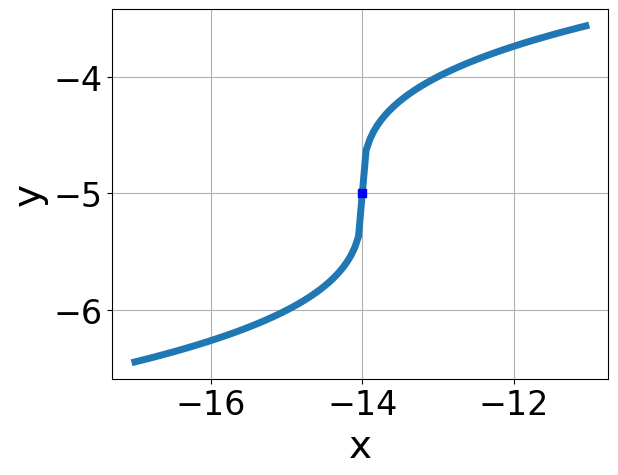
\includegraphics[width=0.5\textwidth]{../Figures/radicalGraphToEquationC.png}
\end{center}
\begin{enumerate}[label=\Alph*.]
\item \( f(x) = - \sqrt[3]{x - 14} - 5 \)
\item \( f(x) = - \sqrt[3]{x + 14} - 5 \)
\item \( f(x) = \sqrt[3]{x - 14} - 5 \)
\item \( f(x) = \sqrt[3]{x + 14} - 5 \)
\item \( \text{None of the above} \)

\end{enumerate} }
\litem{
Choose the graph of the equation below.\[ f(x) = - \sqrt[3]{x + 10} - 3 \]\begin{enumerate}[label=\Alph*.]
\begin{multicols}{2}\item 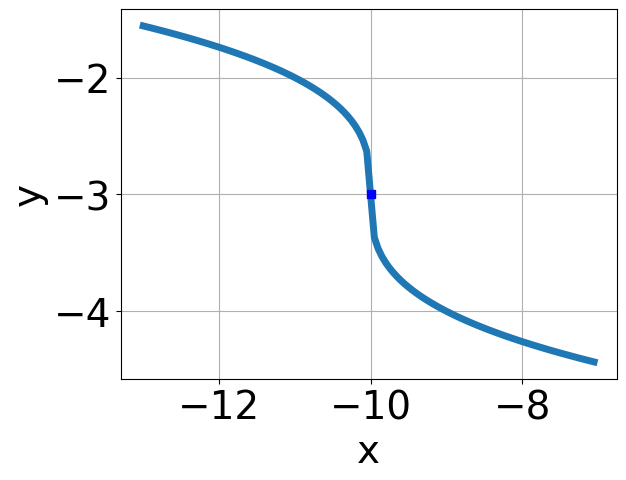
\includegraphics[width = 0.3\textwidth]{../Figures/radicalEquationToGraphCopyAC.png}\item 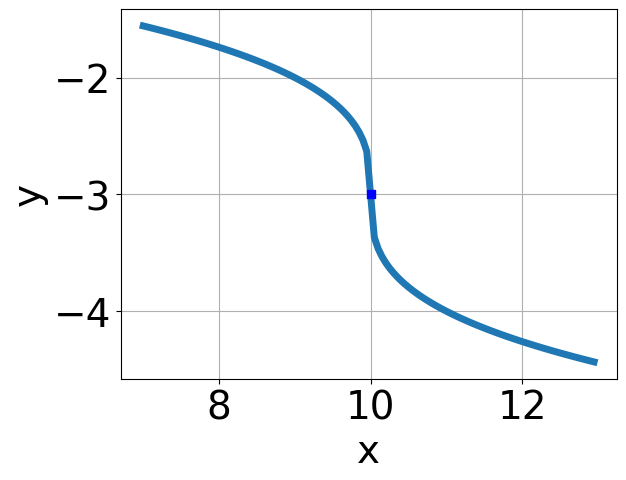
\includegraphics[width = 0.3\textwidth]{../Figures/radicalEquationToGraphCopyBC.png}\item 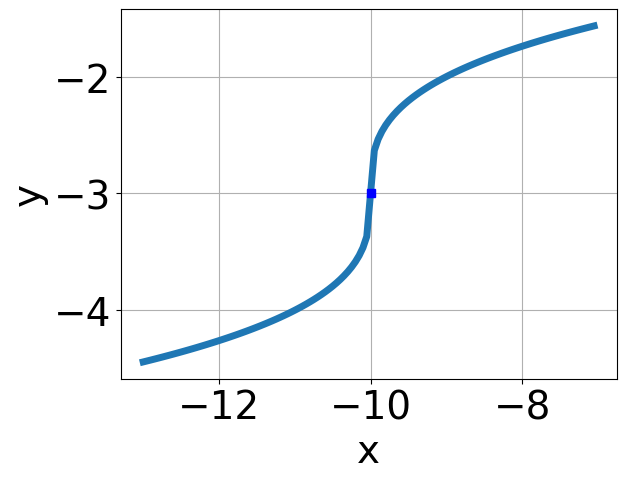
\includegraphics[width = 0.3\textwidth]{../Figures/radicalEquationToGraphCopyCC.png}\item 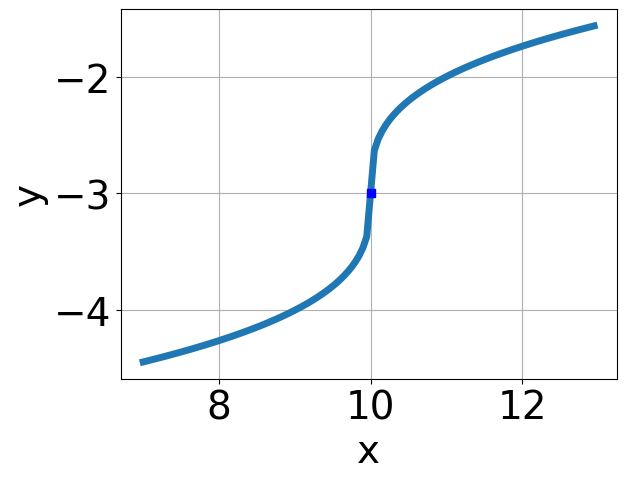
\includegraphics[width = 0.3\textwidth]{../Figures/radicalEquationToGraphCopyDC.png}\end{multicols}\item None of the above.
\end{enumerate} }
\litem{
Choose the graph of the equation below.\[ f(x) = \sqrt[3]{x - 12} + 5 \]\begin{enumerate}[label=\Alph*.]
\begin{multicols}{2}\item 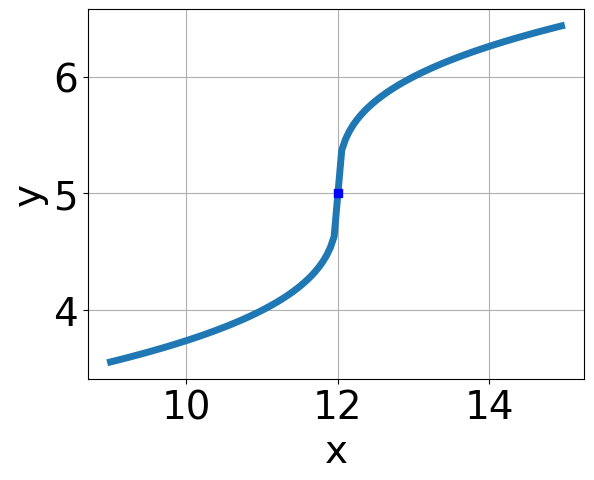
\includegraphics[width = 0.3\textwidth]{../Figures/radicalEquationToGraphAC.png}\item 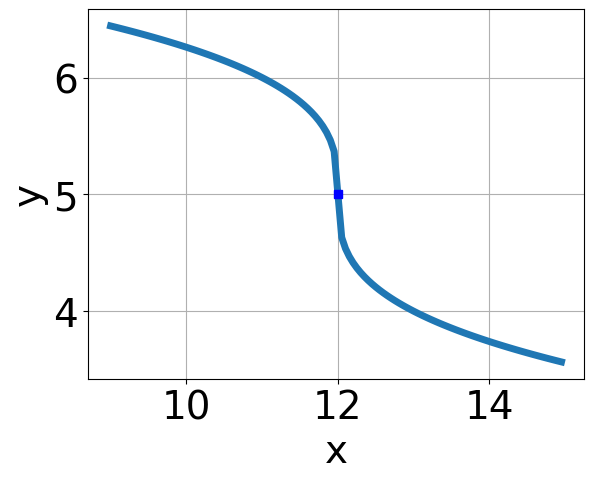
\includegraphics[width = 0.3\textwidth]{../Figures/radicalEquationToGraphBC.png}\item 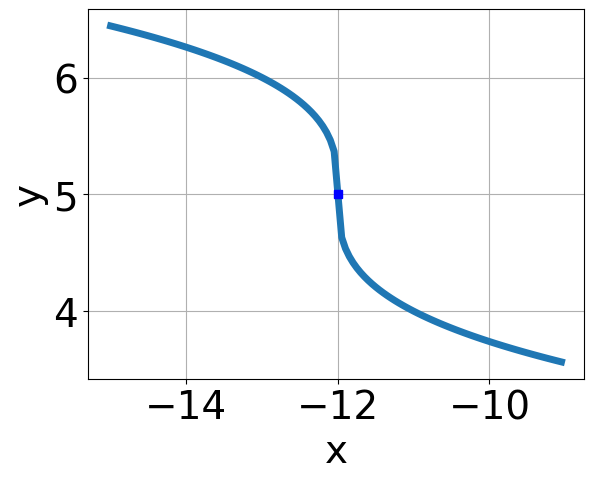
\includegraphics[width = 0.3\textwidth]{../Figures/radicalEquationToGraphCC.png}\item 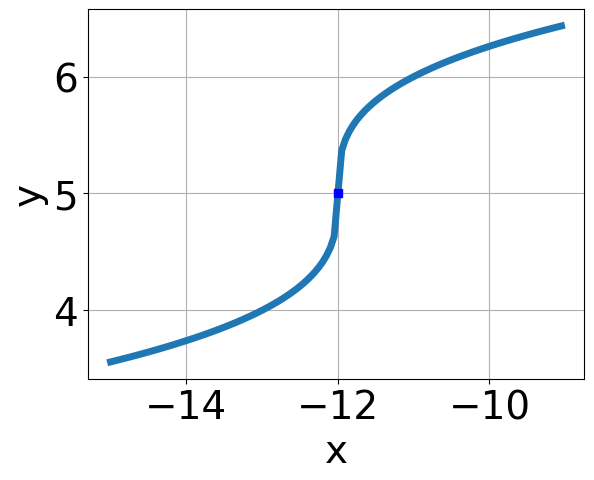
\includegraphics[width = 0.3\textwidth]{../Figures/radicalEquationToGraphDC.png}\end{multicols}\item None of the above.
\end{enumerate} }
\litem{
Solve the radical equation below. Then, choose the interval(s) that the solution(s) belongs to.\[ \sqrt{72 x^2 + 28} - \sqrt{-95 x} = 0 \]\begin{enumerate}[label=\Alph*.]
\item \( x \in [-1.08,-0.68] \)
\item \( x \in [-0.52,0.09] \)
\item \( x_1 \in [0.42, 0.48] \text{ and } x_2 \in [0.4,1.8] \)
\item \( x_1 \in [-1.08, -0.68] \text{ and } x_2 \in [-1,-0.4] \)
\item \( \text{All solutions lead to invalid or complex values in the equation.} \)

\end{enumerate} }
\litem{
Solve the radical equation below. Then, choose the interval(s) that the solution(s) belongs to.\[ \sqrt{-6 x - 7} - \sqrt{-3 x + 3} = 0 \]\begin{enumerate}[label=\Alph*.]
\item \( x_1 \in [-1.28, -0.57] \text{ and } x_2 \in [-1,6] \)
\item \( \text{All solutions lead to invalid or complex values in the equation.} \)
\item \( x \in [-3.86,-3.31] \)
\item \( x \in [-1.63,-1.32] \)
\item \( x_1 \in [-3.86, -3.31] \text{ and } x_2 \in [-4.17,-0.17] \)

\end{enumerate} }
\litem{
Choose the equation of the function graphed below.
\begin{center}
    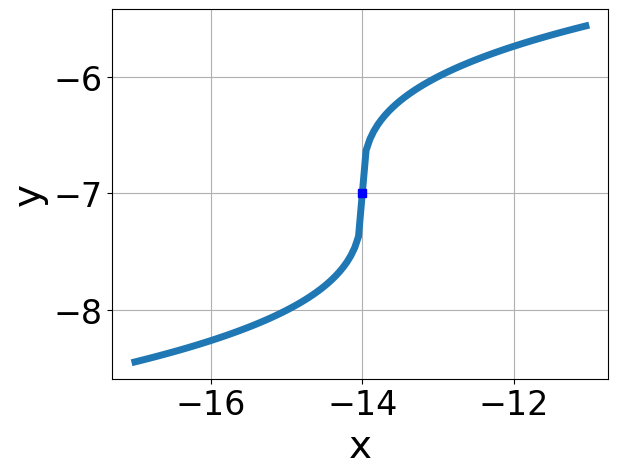
\includegraphics[width=0.5\textwidth]{../Figures/radicalGraphToEquationCopyC.png}
\end{center}
\begin{enumerate}[label=\Alph*.]
\item \( f(x) = \sqrt[3]{x + 14} - 7 \)
\item \( f(x) = - \sqrt[3]{x - 14} - 7 \)
\item \( f(x) = \sqrt[3]{x - 14} - 7 \)
\item \( f(x) = - \sqrt[3]{x + 14} - 7 \)
\item \( \text{None of the above} \)

\end{enumerate} }
\litem{
Solve the radical equation below. Then, choose the interval(s) that the solution(s) belongs to.\[ \sqrt{36 x^2 - 42} - \sqrt{-6 x} = 0 \]\begin{enumerate}[label=\Alph*.]
\item \( \text{All solutions lead to invalid or complex values in the equation.} \)
\item \( x_1 \in [-1, 4] \text{ and } x_2 \in [1.08,1.41] \)
\item \( x \in [-1,4] \)
\item \( x \in [-5.17,0.83] \)
\item \( x_1 \in [-5.17, 0.83] \text{ and } x_2 \in [0.87,1.09] \)

\end{enumerate} }
\litem{
Solve the radical equation below. Then, choose the interval(s) that the solution(s) belongs to.\[ \sqrt{3 x + 9} - \sqrt{-8 x - 9} = 0 \]\begin{enumerate}[label=\Alph*.]
\item \( x \in [-0.5,2.1] \)
\item \( x \in [-2.7,-0.1] \)
\item \( x_1 \in [-5.4, -2.6] \text{ and } x_2 \in [-1.3,1.2] \)
\item \( x_1 \in [-5.4, -2.6] \text{ and } x_2 \in [-3.6,-1.5] \)
\item \( \text{All solutions lead to invalid or complex values in the equation.} \)

\end{enumerate} }
\litem{
What is the domain of the function below?\[ f(x) = \sqrt[6]{-6 x - 4} \]\begin{enumerate}[label=\Alph*.]
\item \( (-\infty, \infty) \)
\item \( [a, \infty), \text{where } a \in [-1.87, -0.88] \)
\item \( [a, \infty), \text{where } a \in [-1.11, -0.03] \)
\item \( (-\infty, a], \text{where } a \in [-2, -0.91] \)
\item \( (-\infty, a], \text{ where } a \in [-1.32, -0.62] \)

\end{enumerate} }
\litem{
What is the domain of the function below?\[ f(x) = \sqrt[4]{-6 x + 7} \]\begin{enumerate}[label=\Alph*.]
\item \( [a, \infty), \text{where } a \in [-0.42, 1.1] \)
\item \( (-\infty, a], \text{ where } a \in [0.98, 1.2] \)
\item \( (-\infty, a], \text{where } a \in [0.83, 0.88] \)
\item \( (-\infty, \infty) \)
\item \( [a, \infty), \text{where } a \in [0.94, 3.35] \)

\end{enumerate} }
\end{enumerate}

\end{document}